\documentclass[11pt]{article}
\usepackage[margin=0.8in]{geometry}
\usepackage{graphicx,booktabs,longtable,tabularx,xcolor,hyperref,enumitem}
\definecolor{ink}{HTML}{17344D}\definecolor{accent}{HTML}{0072B2}
\hypersetup{colorlinks=true,linkcolor=ink,urlcolor=accent,pdftitle={Layerwise benign evaluation across nine supplied saliency-sweep checkpoints},pdfauthor={Pod A saliency study}}
\emergencystretch=2em\setlength{\parindent}{0pt}\setlength{\parskip}{6pt}\setlist{nosep,leftmargin=*}
\renewcommand{\arraystretch}{1.18}
\begin{document}

{\Large\bfseries\color{ink} Layerwise benign evaluation across nine supplied saliency-sweep checkpoints}\par
{\large Verified retain results with recovered, scientifically unqualified forget-related source logs}\par
\textbf{Reporting scope: verified retain evidence; scientific forget integration pending.}\par
\section{Abstract}
We report 42,120 released classifier metric records across nine supplied checkpoints, six benign tasks, all 26 representations, three probe CV partitions and two distinct readout policies. Refitted probes and unchanged original-base probes answer different questions. At both emphasized representations, refitted AUROC exceeds the unchanged readout in 324 of 324 candidate/task/anchor/seed comparisons, with point gaps 0.034778 to 0.503517; 3 existing pointwise intervals include zero. Refitted block 16 AUROC exceeds final normalization descriptively in 162 of 162 candidate/task/seed combinations. Relative to the original pretrained base, results remain task-, layer-, metric- and policy-dependent, including adverse and inconclusive findings. Recovered forget logs contain 23 step-axis validation-loss observations, but no currently qualified scientific aggregate, checkpoint-matched comparison or layerwise forget-performance result. This report completes a bounded reporting scope; the original retain-and-forget request remains partial.\par
\section{Questions and evidence scope}
The scientific questions are whether the six benign labels remain accessible to the chosen linear classifiers, whether the original scaler/readout remains compatible with each supplied endpoint, how those answers vary over representations, and how sequence prediction differs descriptively from classification. The separate forget question requires source qualification that is not established by benign scores or source-log integrity.\par
The reporting plan fixes question-based organization, deterministic candidate/task/layer order, block 16 and final-normalization emphasis, seed 42 as a display convention, and the H3 primary plus multiclass-splice examples. All seeds remain in the complete tables and atlas. Prior outcomes were visible; this reporting plan is not a scientific preregistration. No new experiment, fit, model forward, resampling draw, threshold, calibration or inferential comparison is introduced.\par
\begin{figure}[p]\centering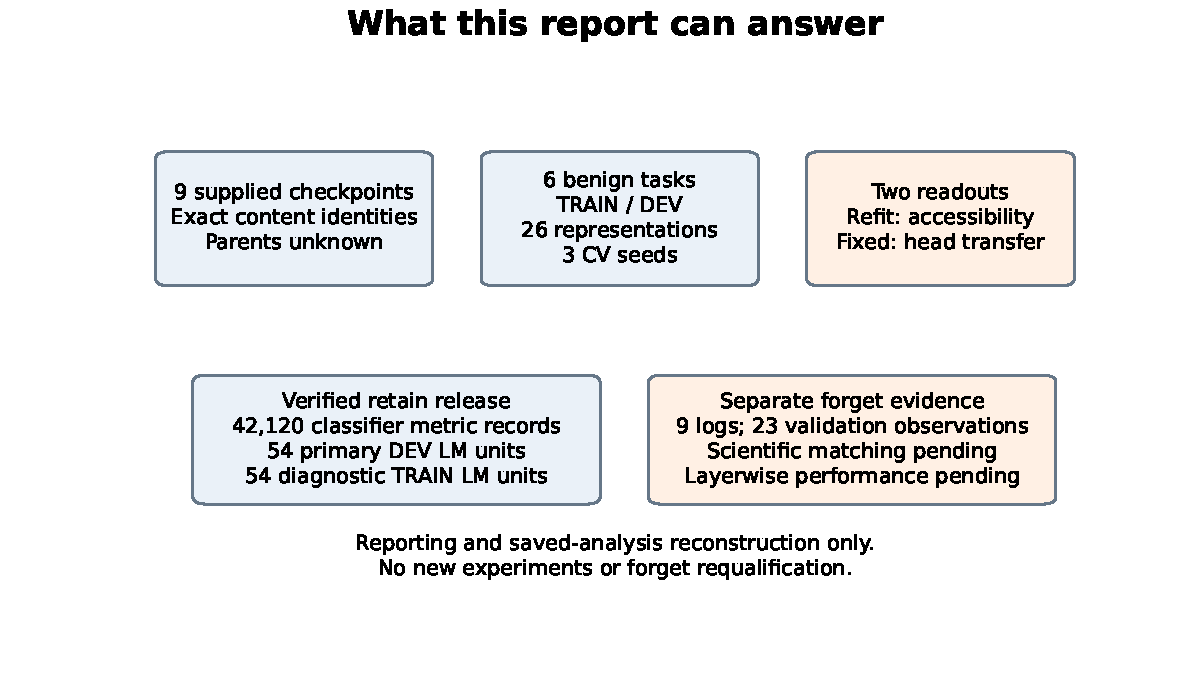
\includegraphics[width=.96\textwidth,height=.79\textheight,keepaspectratio]{figures/STUDY_SCOPE.pdf}\caption{Completed retain-evaluation design and the separate status of source-log forget evidence. CV partitions are not independent intervention replications.}\end{figure}
\section{Checkpoint and task identities}
Registry aliases candidate\_01 through candidate\_09 identify exact delivered tensor content, not old R labels or known intervention parents. Both noise5 endpoints remain distinct at steps 2000 and 2151. Folder labels and nominal percentages describe the supplied naming scheme; they do not prove perturbation masks, realized dose, objective or training exposure. Candidate identities, checkpoint steps and source hashes are retained in every classification table and in \path{REPORTING_FACTS.json}.\par
Tasks are emp\_H3, gue\_tf\_0, gue\_prom\_core\_all, gue\_prom\_300\_all, gue\_splice\_reconstructed and gue\_mouse\_0. Human-readable labels in figures are conservative renderings of these identifiers, not inferred biological aliases. The primary classification split is DEV: H3 has 1497 rows/1497 exact-or-reverse-complement groups; the other tasks have512 rows, with 511 such groups for reconstructed splice. Numeric classes are0/1 for binary tasks and 0/1/2 for splice. No untouched test data were opened.\par
Representations are decoder.layers.0 through decoder.layers.24 and decoder.final\_norm, each width1920 in the qualified extractor. The zero-based decoder.layers.16 is the seventeenth decoder block. Final normalization is a separate representation. All 26 remain available; emphasis is not a global optimum claim.\par
\begin{center}\small
\begin{tabularx}{\textwidth}{lXr}\toprule Alias & Supplied label (not verified mechanism) & Step\\\midrule
candidate\_01 & \path{saliency_maxent_ht_emp_h3_add_noise_top10.0p} & 1500\\
candidate\_02 & \path{saliency_maxent_ht_emp_h3_add_noise_top15.0p} & 1500\\
candidate\_03 & \path{saliency_maxent_ht_emp_h3_add_noise_top20.0p} & 1500\\
candidate\_04 & \path{saliency_maxent_ht_emp_h3_add_noise_top5.0p} & 2000\\
candidate\_05 & \path{saliency_maxent_ht_emp_h3_add_noise_top5.0p} & 2151\\
candidate\_06 & \path{saliency_maxent_ht_emp_h3_reinit_top10.0p} & 1500\\
candidate\_07 & \path{saliency_maxent_ht_emp_h3_reinit_top15.0p} & 1500\\
candidate\_08 & \path{saliency_maxent_ht_emp_h3_reinit_top20.0p} & 1500\\
candidate\_09 & \path{saliency_maxent_ht_emp_h3_reinit_top5.0p} & 1500\\
\bottomrule\end{tabularx}\end{center}
\section{Central analysis pipeline and readout policies}
Previously completed S05--S08 extraction used the qualified frozen native Evo2-1B backend, masked mean nucleotide pooling and preserved tokenizer/preprocessing/loading identities. S09 independently released the saved-output contrasts. S11 derives reporting records from those releases and verification overlays, not from an unverified producer status string. Original producer receipts remain historical; the explicit release overlay controls reuse.\par
Independent refit uses each endpoint's TRAIN features and the frozen balanced L2 logistic-regression procedure. C is selected from 0.1/1/10 using mean fold AUROC, with exact ties going to smaller C. H3 uses three folds; other tasks use five; CV seeds 42/17/1234 identify the recovered fixed StratifiedGroupKFold partitions. Scaling is fold-local during selection and refitted on all TRAIN rows for the final classifier. The established LBFGS tolerance/retry procedure is unchanged. H3 TRAIN has 11971 rows; other TRAIN cohorts have1024 each.\par
Fixed original base applies the exact saved pretrained-base StandardScaler and classifier unchanged to each candidate. It does not recenter, recalibrate, fit a parent head or refit on target features. Refitted performance measures label accessibility under this classifier family and fitting protocol. Fixed-base performance measures compatibility with that original scaler/readout. Neither measures complete task information or proves erasure.\par
The five classifier metrics are AUROC, AP, accuracy, balanced accuracy and classifier cross-entropy. Binary positive class is numeric1 with fixed threshold0.5; multiclass splice uses sorted class order, macro one-vs-rest AUROC, mean classwise AP, argmax accuracy and macro recall. Cross-entropy uses inherited float64-epsilon clipping. AUROC/AP are ranking measures; threshold decisions and probability loss can disagree. Classifier cross-entropy is nats per labeled example. Actual-head LM NLL is nats per valid next-token target and must remain separate.\par
\section{Statistical interpretation}
All admitted comparisons reuse the original2000 exact/RC-group draws, bootstrap seed 20261103, original row/group/class order and explicit common valid-draw masks. Candidate-minus-reference effects are computed within the same draws. Intervals are the original linear 2.5th/97.5th percentiles: 95\% pointwise exploratory intervals conditional on the fitted readouts and cohorts. They omit intervention-training variability and fitting uncertainty and do not provide a familywise guarantee across this grid.\par
An interval crossing zero is inconclusive; it is not equivalence or proof of no change. A positive point is not automatically a confidently positive effect. Seed ranges are descriptive partition sensitivity, not confidence intervals or independent intervention replication. Paired-effect intervals are not obtained by subtracting marginal endpoints. Exact/RC grouping does not establish locus, homology or biological independence.\par
The released inferential inventory is42,120 original-base comparisons,6,480 anchor DNA-control comparisons and 324 anchor policy gaps. The 42,228 deferred specifications remain inactive: 42,120 immediate-parent comparisons and 108 exact LM-base comparisons. Original-base references are qualified comparison baselines, not established immediate parents. Composition and normalized forward4-mer references are simple DNA controls, reused with exact saved heads and cohort/draw associations; outperforming them is not biological understanding.\par
\section{Results: refitting and original-readout compatibility}
At the two fixed anchors, refitted AUROC minus unchanged-base AUROC is positive in 324 of all 324 records. The composition is9 candidates $\times$6 tasks $\times$2 anchors $\times$3 CV seeds. Gaps range from 0.034778 to 0.503517; 3 paired pointwise intervals include zero. These dependent records support a consistent difference between readout policies at the observed anchors, not a causal account of how the intervention changed representations. Evidence: claim policy\_gap.\par
A label can remain accessible after the prescribed refitting procedure even when the original head transfers poorly. This distinction is especially visible on some promoter and TF endpoints. It does not prove all task information is preserved, explain an intervention mechanism or demonstrate relearning. The full all-layer atlas keeps all candidates and all CV partitions rather than selecting the largest gap.\par
\begin{figure}[p]\centering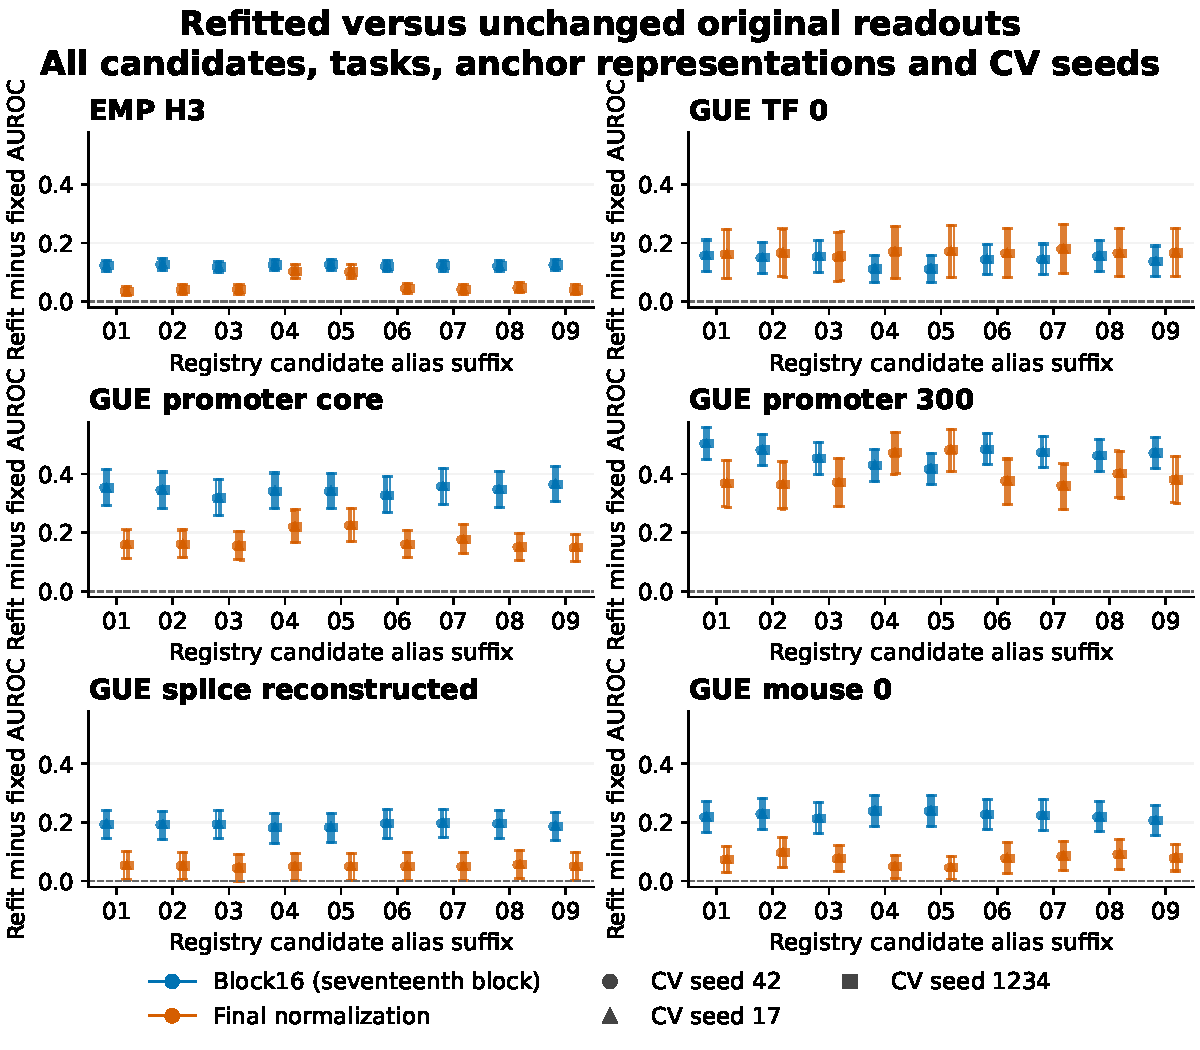
\includegraphics[width=.96\textwidth,height=.79\textheight,keepaspectratio]{figures/ANCHOR_READOUT_GAPS.pdf}\caption{Every candidate, task, anchor and CV seed is shown. Error bars are the already released paired 95\% pointwise conditional intervals. Readout gap is not a universally desirable scientific score.}\end{figure}
\section{Results: representations and all-layer context}
For refitted DEV AUROC, block 16 exceeds final normalization in 162 of 162 candidate/task/CV-seed combinations: 9 $\times$6 $\times$3. This is a descriptive comparison of released point values; no new layer-to-layer test or interval is constructed. It does not establish block 16 as the globally best layer. Evidence: claim anchor\_layer.\par
The complete atlas retains25 decoder-block outputs and final normalization, every classifier metric, both policies and all three CV seeds. Layer shapes and reference-relative effects can vary by task and policy. The atlas uses small multiples and source-linked full-resolution exports; the main report uses the predeclared anchors for readability rather than hiding the intervening layers.\par
\begin{center}\small
\begin{tabularx}{\textwidth}{Xlrr}\toprule Task & Readout & Block16 range & Finalnorm range\\\midrule
EMP H3 & Refit & 0.950469--0.955745 & 0.826702--0.844653\\
EMP H3 & Fixed & 0.827991--0.833874 & 0.725857--0.805337\\
GUE TF 0 & Refit & 0.794531--0.800810 & 0.627805--0.646948\\
GUE TF 0 & Fixed & 0.642594--0.689833 & 0.459232--0.485677\\
GUE promoter core & Refit & 0.838995--0.849020 & 0.766221--0.780642\\
GUE promoter core & Fixed & 0.476744--0.520845 & 0.557041--0.619178\\
GUE promoter 300 & Refit & 0.963775--0.966217 & 0.735515--0.820096\\
GUE promoter 300 & Fixed & 0.461402--0.547448 & 0.335698--0.387106\\
GUE splice reconstructed & Refit & 0.714984--0.732211 & 0.589752--0.614352\\
GUE splice reconstructed & Fixed & 0.527435--0.540307 & 0.540911--0.561017\\
GUE mouse 0 & Refit & 0.821359--0.835527 & 0.640870--0.659298\\
GUE mouse 0 & Fixed & 0.593130--0.616992 & 0.559206--0.611969\\
\bottomrule\end{tabularx}\end{center}
\section{Results: original-base effects include adverse findings}
The reference question differs from the readout-policy question. A refitted candidate can outperform its own unchanged-base readout while still performing below the pretrained-base endpoint. The fixed H3 and multiclass-splice examples use candidate 01, block 16 and CV seed 42; candidate 01 is the first registry alias, not a winner selected by performance.\par
H3 refitted AUROC has candidate-minus-base difference 0.016405 [0.005905, 0.027233]; H3 unchanged-base AUROC has difference -0.105555 [-0.123776, -0.086923]. For splice, the corresponding differences are -0.058885 [-0.094801, -0.023727] and -0.252773 [-0.297963, -0.206501]. Brackets show existing paired 95\% pointwise conditional intervals. These are exact endpoint/reference comparisons, not immediate-parent or selective-unlearning effects. Evidence: the four example claims.\par
Across the full grid there are favorable, adverse, exactly equal and interval-inconclusive comparisons. Summaries in \path{tables/BASE_COMPARISON_SUMMARY.jsonl} preserve task, policy, metric, denominator and exact source IDs. Such row counts are coverage summaries, not percentages of capabilities retained. The 6480 frozen DNA-control contrasts remain reference-specific and anchor-limited; they are not extrapolated into full-layer control inference.\par
\begin{figure}[p]\centering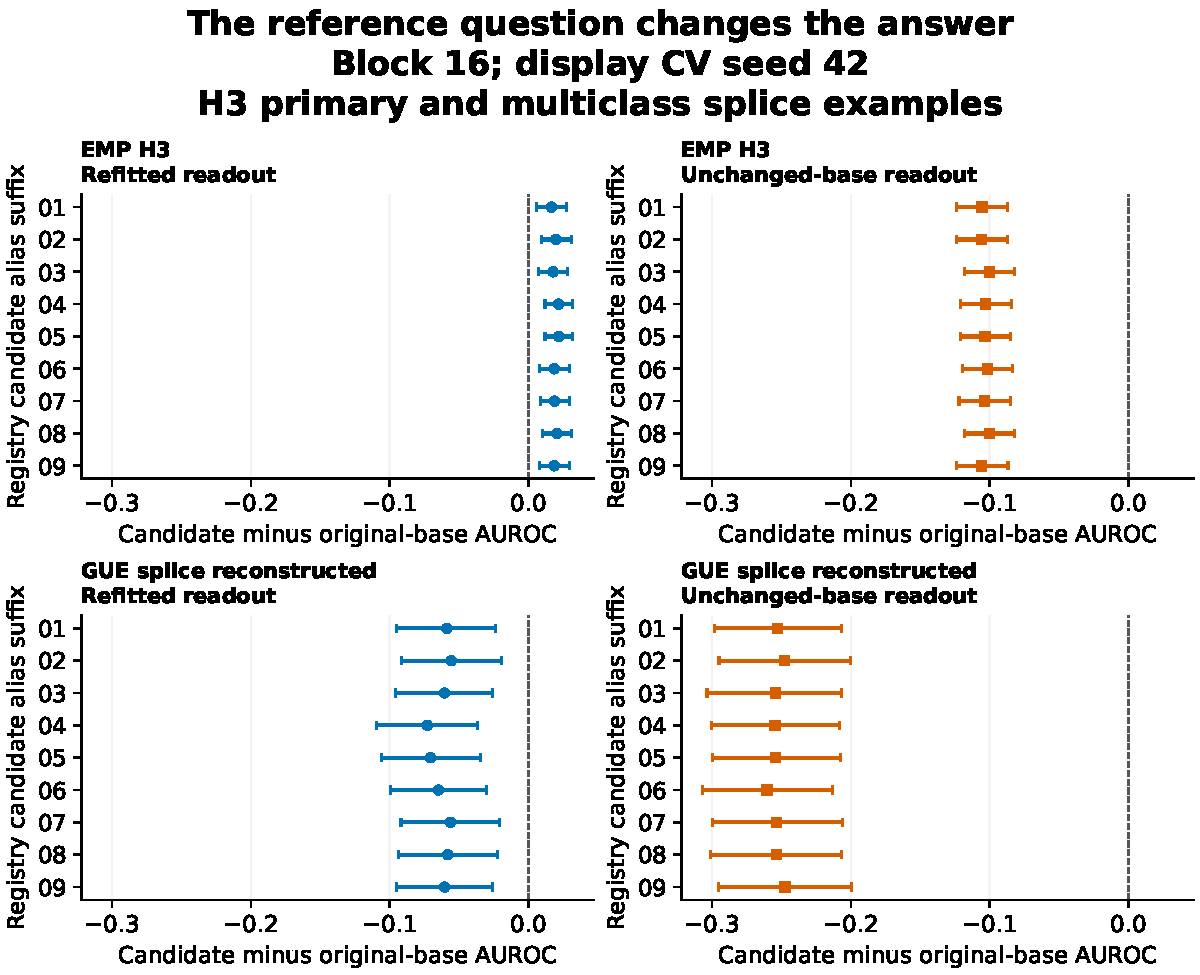
\includegraphics[width=.96\textwidth,height=.79\textheight,keepaspectratio]{figures/ORIGINAL_BASE_EFFECTS.pdf}\caption{All 9 candidate endpoints in fixed H3/splice examples, both readout policies, block 16 and seed 42. Sign is candidate minus original pretrained base. Every adverse and inconclusive interval remains visible.}\end{figure}
\section{Results: ranking, probability quality and seed sensitivity}
At 220 of 8,424 candidate/task/representation/seed/policy cells, AUROC is above the base point while classifier cross-entropy is worse (higher). This descriptive conjunction shows that ranking and probability quality cannot substitute for each other. It is not a joint-significance test or capability percentage. Exact paired source IDs are in \path{tables/RANKING_LOSS_DISAGREEMENT.jsonl}. Evidence: claim ranking\_loss.\par
Different CV partitions can select the same C and therefore the same final all-TRAIN fit. The inherited seed-sensitivity table exposes coincident values and sign exceptions without choosing the favorable partition. Repeated final heads or predictions do not create independent intervention replications. All source seed groups remain in \path{REPORTING_FACTS.json} and the S09 all-layer atlas.\par
\section{Results: sequence prediction is separate}
The 108 LM units comprise54 primary DEV and 54 diagnostic TRAIN units: 9 candidates $\times$6 tasks $\times$2 splits. They produce216 NLL/perplexity metric records. They are not 108 independent held-out evaluations and are not expanded across probe layers or CV seeds. DEV uses its existing conditional group-bootstrap intervals. TRAIN diagnostics have no invented uncertainty.\par
Perplexity is exp(aggregated NLL) under the qualified actual output head and valid-target mask. The report does not average across tasks or combine LM loss with classifier cross-entropy. Different task cohorts can exhibit different sequence-prediction losses alongside different classification profiles; this is descriptive coexistence, not a new correlation, causal association or combined capability score. LM original-base comparisons remain deferred, so the figure does not claim an improvement relative to base or parent.\par
\begin{figure}[p]\centering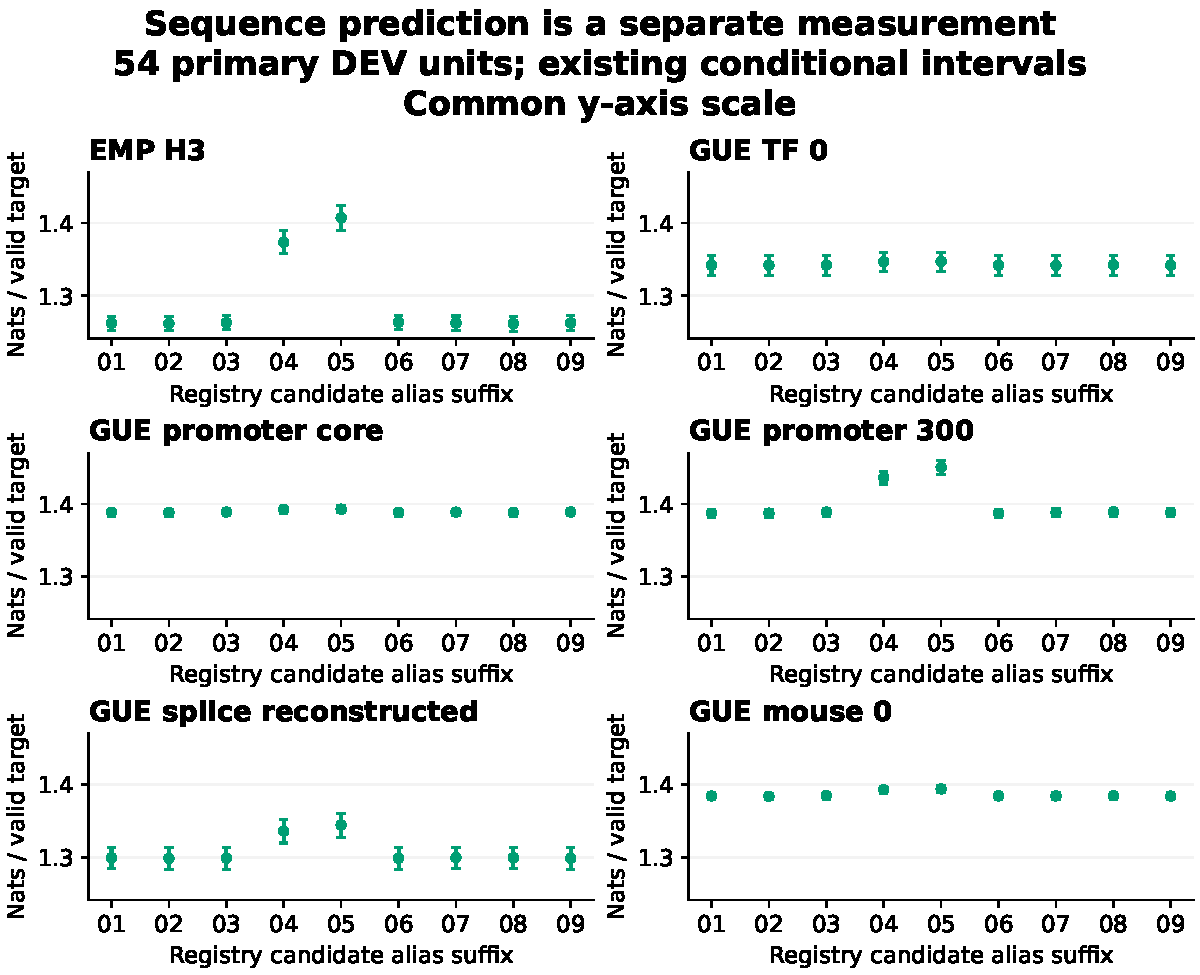
\includegraphics[width=.96\textwidth,height=.79\textheight,keepaspectratio]{figures/LM_DEV_RESULTS.pdf}\caption{All 54 primary DEV LM NLL units with existing intervals. Candidate aliases remain categorical; no connected dose trajectory or independent-seed interpretation is introduced. All panels use the same y-axis scale.}\end{figure}
\begin{center}\small
\begin{tabularx}{\textwidth}{Xrr}\toprule Task & DEV NLL range & DEV perplexity range\\\midrule
EMP H3 & 1.261821--1.407216 & 3.531848--4.084568\\
GUE TF 0 & 1.341846--1.347291 & 3.826101--3.846989\\
GUE promoter core & 1.388296--1.392800 & 4.008016--4.026109\\
GUE promoter 300 & 1.386966--1.450487 & 4.002689--4.265191\\
GUE splice reconstructed & 1.298836--1.344685 & 3.665030--3.836976\\
GUE mouse 0 & 1.384227--1.394259 & 3.991738--4.031987\\
\bottomrule\end{tabularx}\end{center}
\section{Corrected forget-evidence assessment}
Forget-related source logs were supplied and recovered. Corrective S10 verified nine event files,418,914,867 source bytes,4,069,391 complete events and 4,069,382 scalar observations. There are14,090 step-axis training forget-loss observations,23 step-axis forget-validation-loss observations and 23 corresponding step-axis logged validation-ppl values. The 92 loss/ppl/both-axis records are not 92 independent validation evaluations. Alternate sample-axis series repeat the same observations; nine files are not nine independent training runs.\par
Reinit5 A contains two distinct forget loss validation values at step 1500: 1.3953843116760254 and 1.3952388763427734. Both remain present; neither is averaged away or selected as the last call. Reinit5 B records training only through 1439 with a different validation history. Noise5 step 2000 and 2151 are distinct delivered endpoints with unresolved exact log-to-content binding, not independent seeds. Configurations declare702 versus 1 evaluation iterations, but this does not establish the actual unique-example/valid-target denominator, distributed reduction, masking or exposure.\par
Transport and scalar extraction are verified, but exact checkpoint/invocation, metric definition/direction, cohort/split, denominator/aggregation and producing implementation identities remain unqualified. Thus there are zero currently qualified scientific forget aggregates, zero checkpoint-matched comparisons and zero qualified layerwise forget-performance observations. Layer-indexed gradient norms are optimization diagnostics. A model-level loss cannot be copied across26 layers to satisfy a layerwise request. Evidence: claim source\_forget and the unchanged corrected S10 ledger.\par
The 9 $\times$26 representation slots are only a coverage illustration. A full forget task, split, metric, readout, policy and seed dimensions grid is unspecified; no project completion percentage or fabricated missing-cell denominator is supplied. No retain/forget frontier, successful forgetting, causal selectivity or optimal checkpoint is inferred from source logs. Original scalar names are not relabeled as verified biological metrics or held-out NLL.\par
\begin{figure}[p]\centering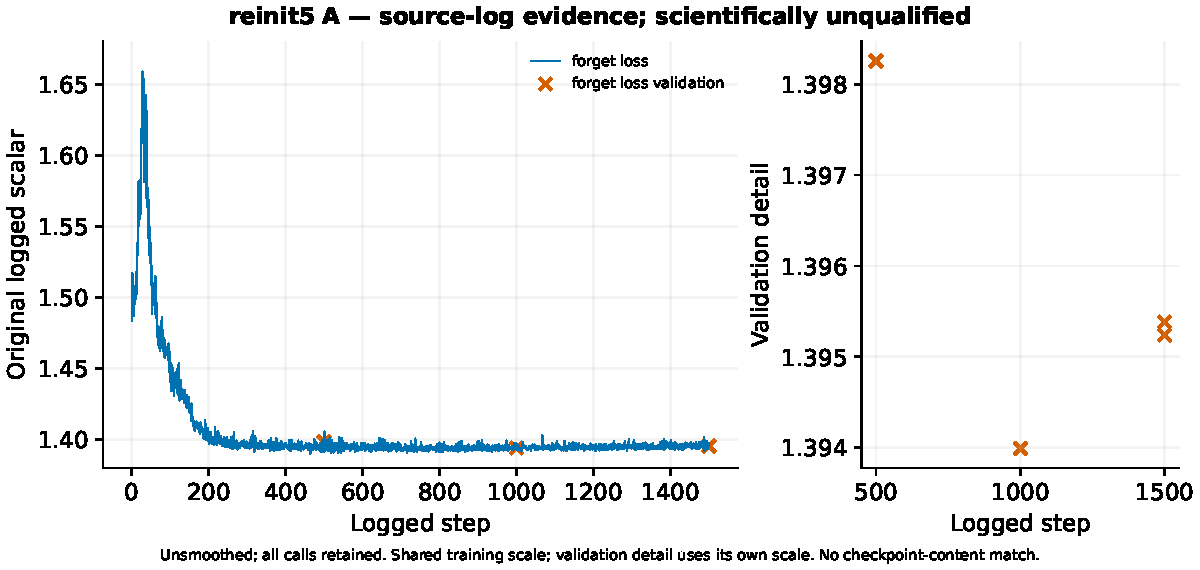
\includegraphics[width=.96\textwidth,height=.79\textheight,keepaspectratio]{figures/FORGET_SOURCE_REINIT5_A.pdf}\caption{Source-log evidence; scientifically unqualified. Reinit5 A unsmoothed training and all 4 validation observations, including both step 1500 values. The complete gallery includes readable individual panels for all 9 logs and the unchanged full S10 overview.}\end{figure}
\section{Limitations tied to claims}
Unknown immediate parents block intervention-parent effects; comparisons with the qualified original pretrained base remain valid at their actual descriptive reference scope. Unverified saliency masks, perturbation laws and realized doses block mechanistic or calibrated-strength comparisons; the supplied endpoint measurements remain valid. Endpoint-step/exposure differences block controlled dose-response or method attribution; both noise5 identities remain separate.\par
Independent intervention replication is not established. Probe CV seeds and source files cannot fill that gap; conditional readout/cohort descriptions remain valid. Unqualified forget semantics and content binding block scientific retain/forget integration; source integrity, original-tag quotations and duplicate diagnostics remain usable. Missing layerwise forget performance blocks the original layerwise combined conclusion; it does not invalidate the verified layerwise benign measurements.\par
Whole-delivery inventory remains PARTIAL, so nine selected endpoints are not an exhaustive sweep claim. Candidate 05 historical upload privacy remains unknown; current private protection is verified separately and cannot retroactively establish original visibility. Recovery verifies exact archived bytes and the declared sampled saved-analysis panel, not all model execution, biological truth, fresh GPU replay or a clean scientific-runtime rebuild. R2 was not produced and is excluded. Pod B relearning remains separate. No-deadline continuity is preserved.\par
\section{Reproducibility and future evidence intake}
\path{REPORTING_FACTS.json} is the common numerical source for this report, the reviewer briefing, tables and new figures. \path{CLAIM_LEDGER.jsonl} binds every headline and fixed numerical example to exact source IDs, scope, metric direction, intervals or explicit lack of uncertainty, and interpretation limits. \path{TABLE_INDEX.json} gives full-precision table paths and hashes; \path{FIGURE_SOURCE_MAP.json} binds individual displayed coordinates to source keys; \path{FIGURE_GALLERY.md} indexes the complete immutable atlas.\par
Fresh CPU recovery uses the unchanged original S05 and S08 saved-head selectors: 252 paths spanning every candidate/task, both policies, both emphasized representations and all CV seeds across the panel, including multiclass splice. The full seed crossproduct is not crossed within each unit. Saved scalers/heads and selected features reproduce probabilities; original draws reproduce metrics/vectors/intervals. Tolerances remain absolute 1e-10 for probabilities and 1e-12 for metric/draw/interval values, relative zero. See \path{FRESH_CPU_RESTORE_CHECK.json} for actual scope, worst residuals and locations; byte verification, sampled numerical reconstruction, reporting regeneration, unperformed GPU replay and unperformed clean-runtime recreation are explicitly separate.\par
New checkpoint/log invocation bindings or evaluation/cohort/aggregation metadata require a separately versioned S10 qualification assessment. Compatible reference aggregates affect only eligible reference claims. Genuine layerwise aggregates require their own task/readout/hook/protocol qualification. A corrected source creates a new immutable source version and invalidates only its dependent joins/claims/figures; unaffected retain science remains reusable. The concise collaborator request remains unsent. No future stage or workflow starts automatically.\par
\section{Conclusion}
Under the chosen frozen classifier family, benign label accessibility after refitting and compatibility with the original readout are distinct empirical properties. Their differences vary across tasks and representations and coexist with adverse, flat and inconclusive original-base results. Sequence prediction is a separate task-specific measurement. The recovered forget logs establish supplied source observations, not qualified forgetting or layerwise forget performance. Reporting can finish for this evidence scope while the original retain-and-forget request remains partial.\par
\section*{Complete evidence and source links}
\href{TABLE_INDEX.json}{Full-precision tables and source identities}; \href{CLAIM_LEDGER.jsonl}{claim ledger}; \href{FIGURE_GALLERY.md}{complete figure gallery}; \href{FRESH_CPU_RESTORE_CHECK.json}{fresh CPU recovery scope and exact residual locations}; \href{FINAL_RECEIPT.json}{actual delivery identities}.
\end{document}
